%%%%%%%%%%%%%%%%%%%%%%%%%%%%%%%%%%%%%%%%%
% Beamer Presentation
% LaTeX Template
% Version 1.0 (10/11/12)
%
% This template has been downloaded from:
% http://www.LaTeXTemplates.com
%
% License:
% CC BY-NC-SA 3.0 (http://creativecommons.org/licenses/by-nc-sa/3.0/)
%
%%%%%%%%%%%%%%%%%%%%%%%%%%%%%%%%%%%%%%%%%

%----------------------------------------------------------------------------------------
%	PACKAGES AND THEMES
%----------------------------------------------------------------------------------------

\documentclass{beamer}

\mode<presentation> {

% The Beamer class comes with a number of default slide themes
% which change the colors and layouts of slides. Below this is a list
% of all the themes, uncomment each in turn to see what they look like.

%\usetheme{default}
%\usetheme{AnnArbor}
%\usetheme{Antibes}
%\usetheme{Bergen}
%\usetheme{Berkeley}
%\usetheme{Berlin}
%\usetheme{Boadilla}
\usetheme{CambridgeUS}
%\usetheme{Copenhagen}
%\usetheme{Darmstadt}
%\usetheme{Dresden}
%\usetheme{Frankfurt}
%\usetheme{Goettingen}
%\usetheme{Hannover}
%\usetheme{Ilmenau}
%\usetheme{JuanLesPins}
%\usetheme{Luebeck}
%usetheme{Madrid}
%\usetheme{Malmoe}
%\usetheme{Marburg}
%\usetheme{Montpellier}
%\usetheme{PaloAlto}
%\usetheme{Pittsburgh}
%\usetheme{Rochester}
%\usetheme{Singapore}
%\usetheme{Szeged}
%\usetheme{Warsaw}

% As well as themes, the Beamer class has a number of color themes
% for any slide theme. Uncomment each of these in turn to see how it
% changes the colors of your current slide theme.

%\usecolortheme{albatross}
%usecolortheme{beaver}
%\usecolortheme{beetle}
%\usecolortheme{crane}
%\usecolortheme{dolphin}
%\usecolortheme{dove}
%\usecolortheme{fly}
%\usecolortheme{lily}
%usecolortheme{orchid}
%\usecolortheme{rose}
%\usecolortheme{seagull}
\usecolortheme{seahorse}
%\usecolortheme{whale}
%\usecolortheme{wolverine}

%\setbeamertemplate{footline} % To remove the footer line in all slides uncomment this line
%\setbeamertemplate{footline}[page number] % To replace the footer line in all slides with a simple slide count uncomment this line

\setbeamertemplate{navigation symbols}{} % To remove the navigation symbols from the bottom of all slides uncomment this line
}
%\usepackage[brazilian]{babel}
\usepackage[utf8]{inputenc}
\usepackage{pgfplots}
\usepackage{graphicx} % Allows including images
\usepackage{booktabs} % Allows the use of \toprule, \midrule and \bottomrule in tables
\usepackage{courier}
%----------------------------------------------------------------------------------------
%	TITLE PAGE
%----------------------------------------------------------------------------------------

\title[EP2]{EP2 de MAC0422} % The short title appears at the bottom of every slide, the full title is only on the title page

\author{Gabriel Capella e Luís Felipe de Melo} % Your name
\institute[USP] % Your institution as it will appear on the bottom of every slide, may be shorthand to save space
{
Universidade de São Paulo \\ % Your institution for the title page
\medskip
}

\begin{document}

\begin{frame}
\titlepage % Print the title page as the first slide
\end{frame}

%----------------------------------------------------------------------------------------
%	PRESENTATION SLIDES
%----------------------------------------------------------------------------------------

%------------------------------------------------
%\section{Problema} % Sections can be created in order to organize your presentation into discrete blocks, all sections and subsections are automatically printed in the table of contents as an overview of the talk
%------------------------------------------------

%\subsection{Subsection Example} % A subsection can be created just before a set of slides with a common theme to further break down your presentation into chunks

\begin{frame}
\frametitle{Problema}
Temos que simular uma das provas do ciclismo, a perseguição por equipe. No programa, temos 2 equipes, e cada uma possui \texttt{n} ciclistas. A pista possui \texttt{d} metros. Cada time começa em um lado oposto da pista. Durante a corrida, apenas dois ciclistas podem estar lado a lado no circuito. Vence a equipe cujo terceiro ciclista ultrapassa o terceiro ciclista da outra equipe ou quando o terceiro ciclista de uma equipe termina 16 voltas primeiro.\\~\\

\end{frame}

\begin{frame}
\frametitle{Implementação}	
\begin{itemize}
\item Cada ciclista é implementado com uma thread \texttt{ciclista}. 
\item Implementamos a pista como dois vetores de tamanho \texttt{2*d} (logo, cada ciclista ocupa duas posições no vetor). Os dois vetores representam a pista interna e a pista externa.
\item Fizemos essa escolha porque as velocidades podem variar, no modo \texttt{v}. 
\item Então, quando o ciclista está a 30 km/h, ele se move uma posição no vetor. Quando está a 60 km/h, move-se duas.
\item Temos um "juiz" que fiscaliza a corrida.
\end{itemize}
\end{frame}

%------------------------------------------------
\begin{frame}
\frametitle{Considerações}
\begin{itemize}
	\item O custo da ultrapassagem (sair da pista interna e ir para a externa) é o mesmo custo de ir para a frente.
	\item Cada ciclista é autônomo, ele sabe as regras e decide se ultrapassa ou não.
	\item A corrida começa com todos os ciclistas fora da pista e os ciclistas da equipe A são inseridos nas posições 0 e 1 (já que em nossa implementação os ciclistas ocupam duas posições de vetor) do vetor e os ciclistas da equipe B são inseridos nas posições \texttt{d} e \texttt{d+1}.
	
\end{itemize}
\end{frame}

\begin{frame}
	\begin{itemize}
		\item Sobre o ciclista que “segura” os outros:  quando um ciclista passar na linha de chegada, ele vai ver se existe algum colega de equipe com número de voltas maior do que o dele em sua frente e que tenha a velocidade de 30km/h.  Se ninguém tiver ele sorteia a velocidade, se alguém tiver ele vai andar a 30 km/h.
		\item Quando dois ciclistas paralelos a 60 km/h se deparam com um ciclista a 30 km/h à frente, o primeiro que conseguir o mutex para ficar paralelo ao de 30 km/h vai manter a velocidade. O outro vai ficar a 30 km/h.
	\end{itemize}
\end{frame}
%------------------------------------------------
\begin{frame}
	\frametitle{Probabilidade de quebra}
	\begin{itemize}
		\item Temos no enunciado que a probabilidade de quebra é 10\% e 4 rodadas. 
		Vamos considerar que ela seja uniforme, ou seja, a probabilidade de quebrar em movimento será: \\
		\begin{center} 
			$P(q) = \frac{0,1 \cdot v}{n \cdot d \cdot 8}$
		\end{center}
		\item Onde v é a velocidade, que é 1 caso 30 km/h ou 2, caso contrário.
		\item Exemplo: Um ciclista está andando a 60 km/h. A probabilidade de que ele quebre a cada passo da iteração em uma pista de 400 m é de 0.00125.
		\item Obs: O ciclista anda e quebra, não começa uma volta quebrado, mas pode terminar assim. 
		
	\end{itemize}
\end{frame}

\begin{frame}
	\begin{itemize}
		\item Em nosso código, utilizamos o tempo como raiz da função \texttt{random}.
		\item Temos a seguinte fórmula:
		\begin{center} 
			$P(q) = \frac{speed}{n \cdot d \cdot 80}$
		\end{center}
		\item Note que duas vezes a distância máxima é igual à máxima posição que um ciclista pode estar, portanto o 40 da nossa fórmula.
	\end{itemize}
\end{frame}

%------------------------------------------------
\begin{frame}
	\frametitle{Módulos}
	\framesubtitle{barrier.c}
	\begin{itemize}
		\item Fizemos a nossa própria biblioteca de barreiras. 
		\item A principal razão disso é que as barreiras da \texttt{pthread.h} não funcionariam direito quando um ciclista quebra. Quando ele quebra, sua thread é destruída, e o número de threads é alterado.
		\item Implementamos nossa barreira como uma struct que possui dois semáforos (mutexes), uma variável condicional das pthreads o número total de threads e um contador de quantas já finalizaram.
		\item Existem as funções de inicializar, destruir, esperar e a remover uma thread.
	\end{itemize}
\end{frame}

\begin{frame}
	\frametitle{Módulos}
	\framesubtitle{cyclist.c}
	\begin{itemize}
		\item Esse módulo cuida de tudo relacionado aos ciclistas.
		\item Declaramos o ciclista como uma
		\texttt{struct} que possui os seguintes campos:
		\begin{itemize}
			\item Número do ciclista.
			\item Número do time.
			\item A distância total percorrida.
			\item Status do ciclista.         
			\item Velocidade.
			\item Qual pista ele está.
			\item Momento em que acaba a prova.
			\item Qual a linha de chegada dele.    
			\item Qual volta ele está.     
			\item Se o inspetor validou a volta dele.
		\end{itemize}
	\end{itemize}	
\end{frame}

\begin{frame}
	\begin{itemize}
		\item Esse módulo possui funções públicas e privadas.
		\item As funções públicas são as de configurar o ambiente, inicializar o ciclista, a função para a thread do ciclista e a função de desalocar a memória.
		\item As funções privadas são as funções de ver como está a frente do ciclista (posição e semáforo mutex), a de colocar o ciclista na pista e a de avançar \texttt{x} posições. 
	\end{itemize}
\end{frame}

\begin{frame}
	\frametitle{Módulos}
	\framesubtitle{inspector.c}
	\begin{itemize}
		\item Esse módulo funciona como um juiz para a prova.
		\item É como se tivesse alguém responsável por ver se a corrida está indo de forma correta.
		\item Suas funções são: mostrar quem quebrou, exibir os dados do fim da corrida e dizer se o ciclista pode acelerar (de 30 km/h para 60 km/h).
		\item Ele possui uma função de inicialização (basicamente pegando as informações que vieram da \texttt{main}) e uma que checa as seguintes informações:
		\begin{itemize}
			\item O número de voltas.
			\item O decremento da barreira.
			\item Como estão os terceiros das equipes (se terminou a corrida ou se passou na frente do outro terceiro).
		\end{itemize}
	\end{itemize}	
\end{frame}

\begin{frame}
	\frametitle{Módulos}
	\framesubtitle{ep2.c}
	\begin{itemize}
		\item Recebe as informações da entrada e assim define as modos de execução, passando essas informações para as funções dos módulos.
		\item Declara o espaço de trabalho, chama as funções de inicialização e então convoca as de execução para os ciclistas.
		\item Usa as funções do juiz para exibição de informações.
	\end{itemize}	
\end{frame}

\begin{frame}
	\frametitle{Simulador}
	\begin{itemize}
		\item Para ver se nossa implementação foi feita corretamente, fizemos um simulador para averiguar se a corrida estava coerente. 
		\item Os resultados estão a seguir:
	\end{itemize}
\end{frame}

\begin{frame}
	\begin{figure}[!h]
		\centering
		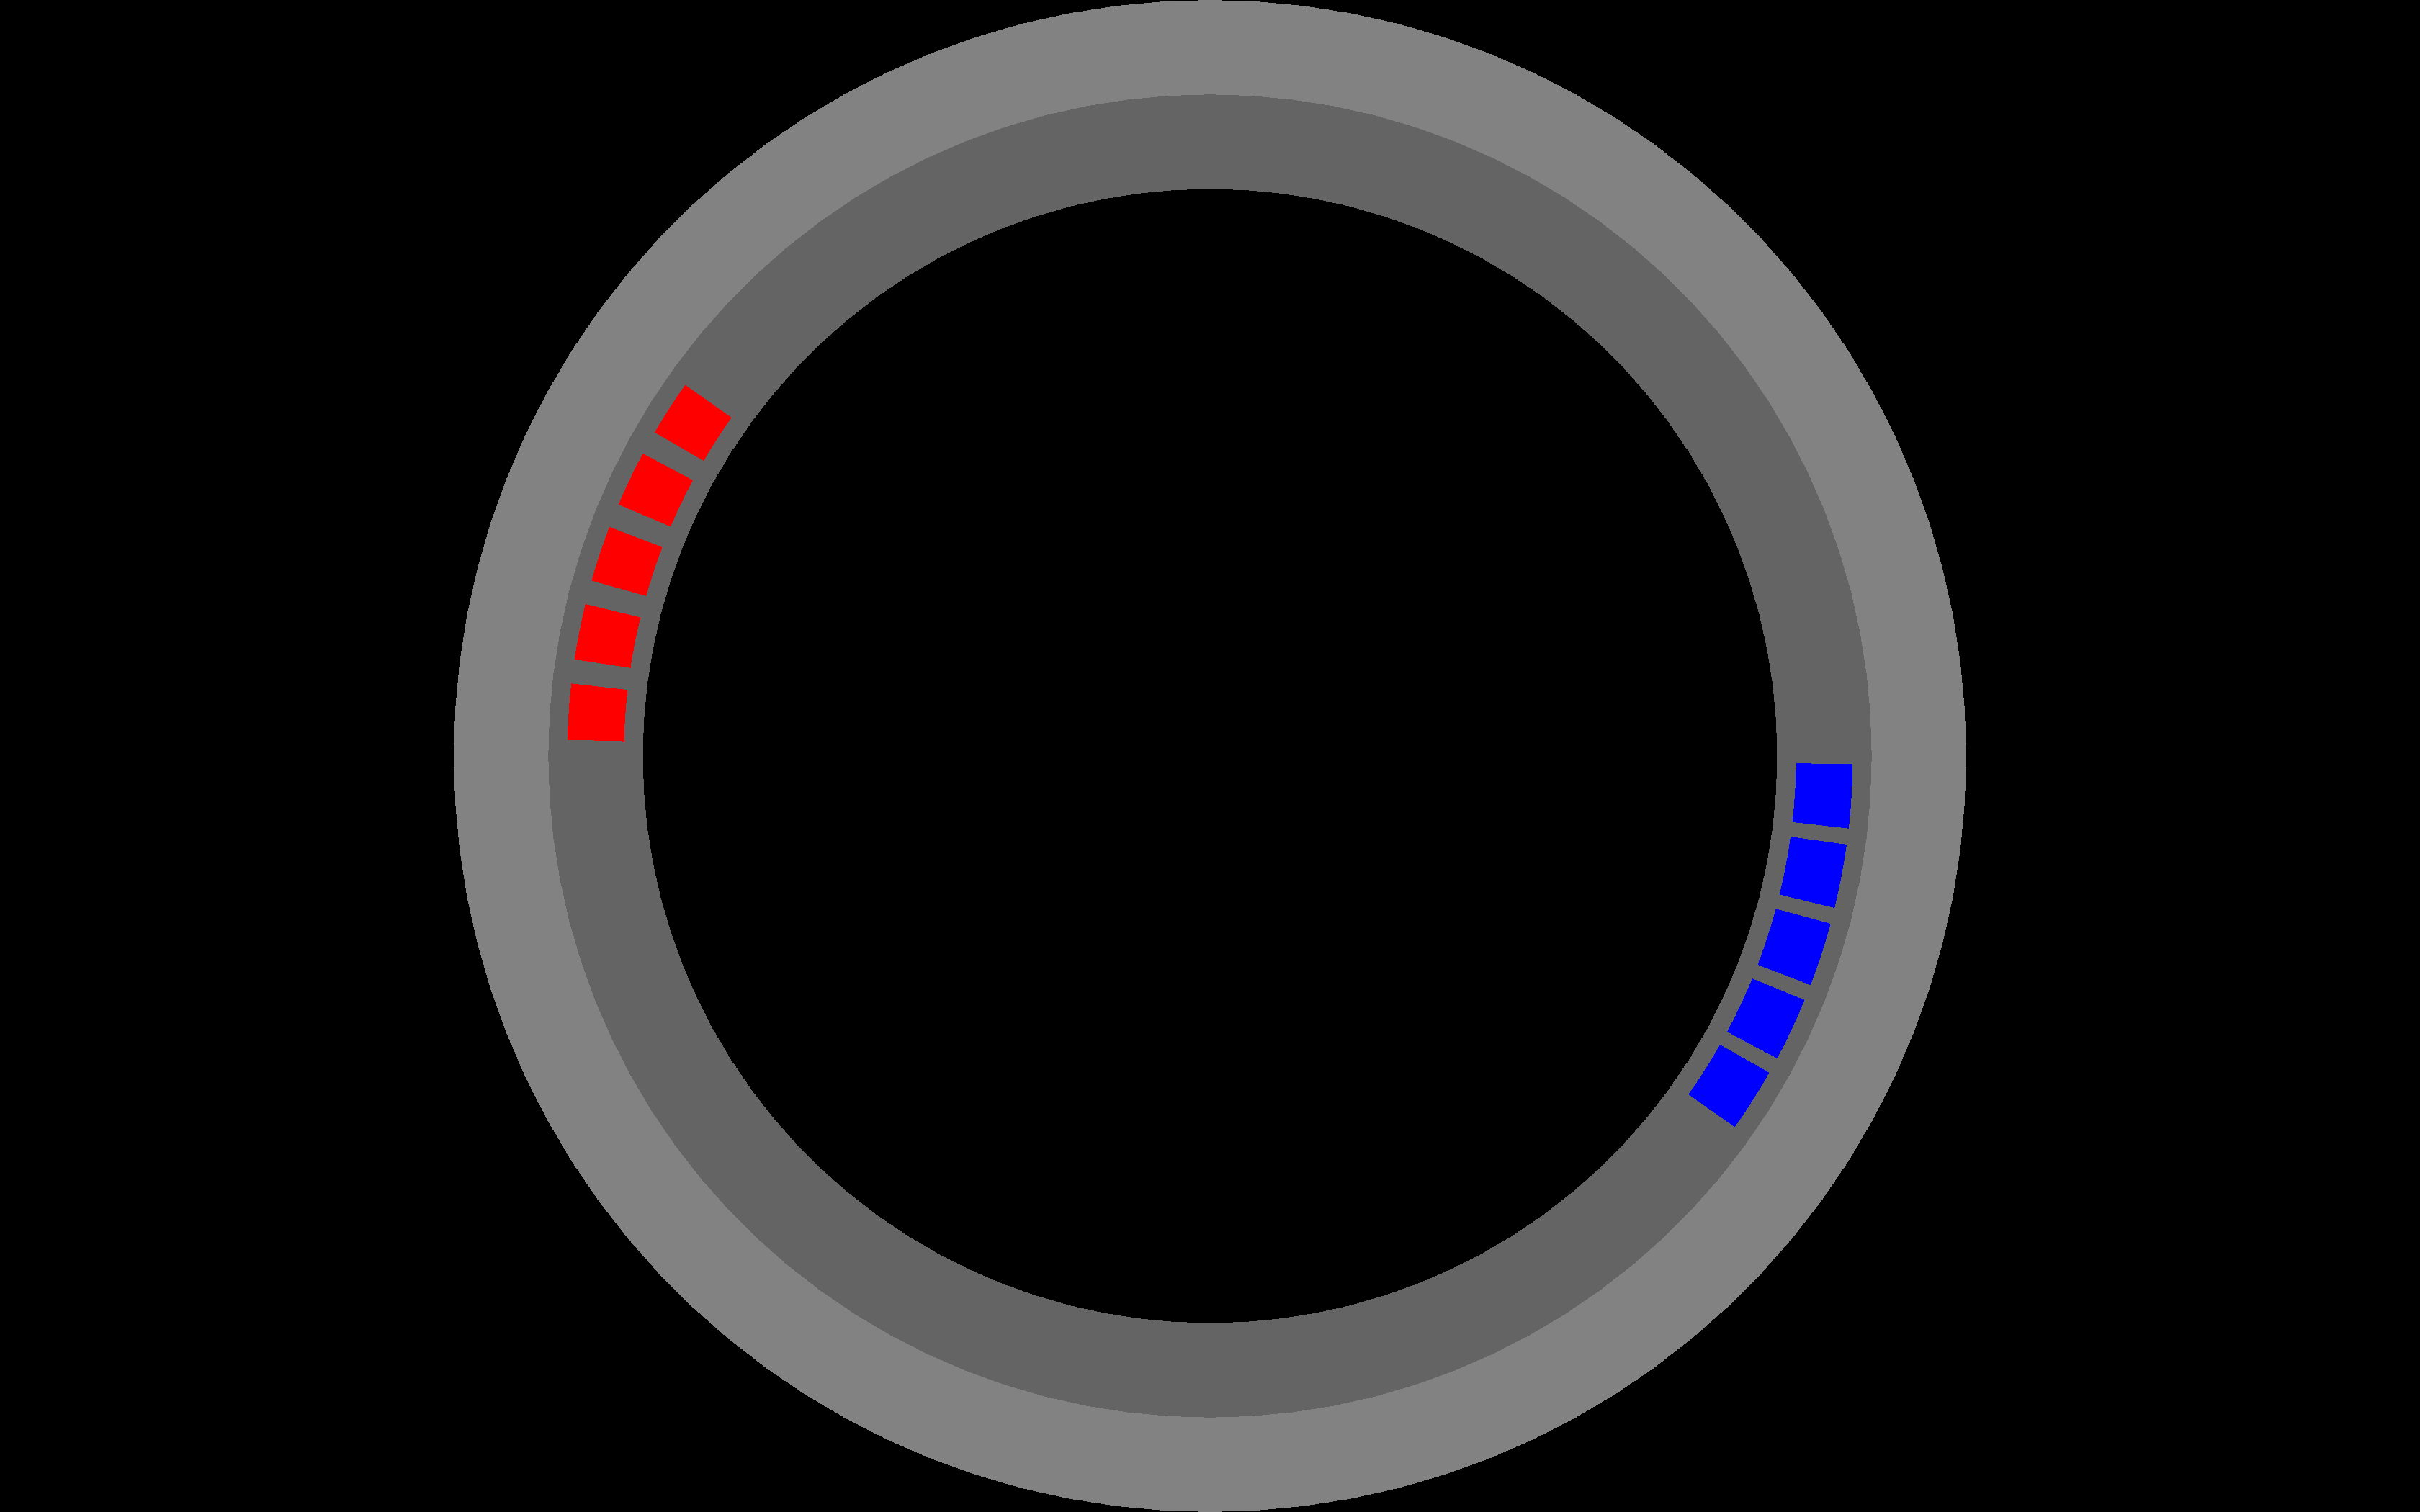
\includegraphics[scale=0.2]{10.png}
	\end{figure}
\end{frame}

\begin{frame}
	\begin{figure}[!h]
		\centering
		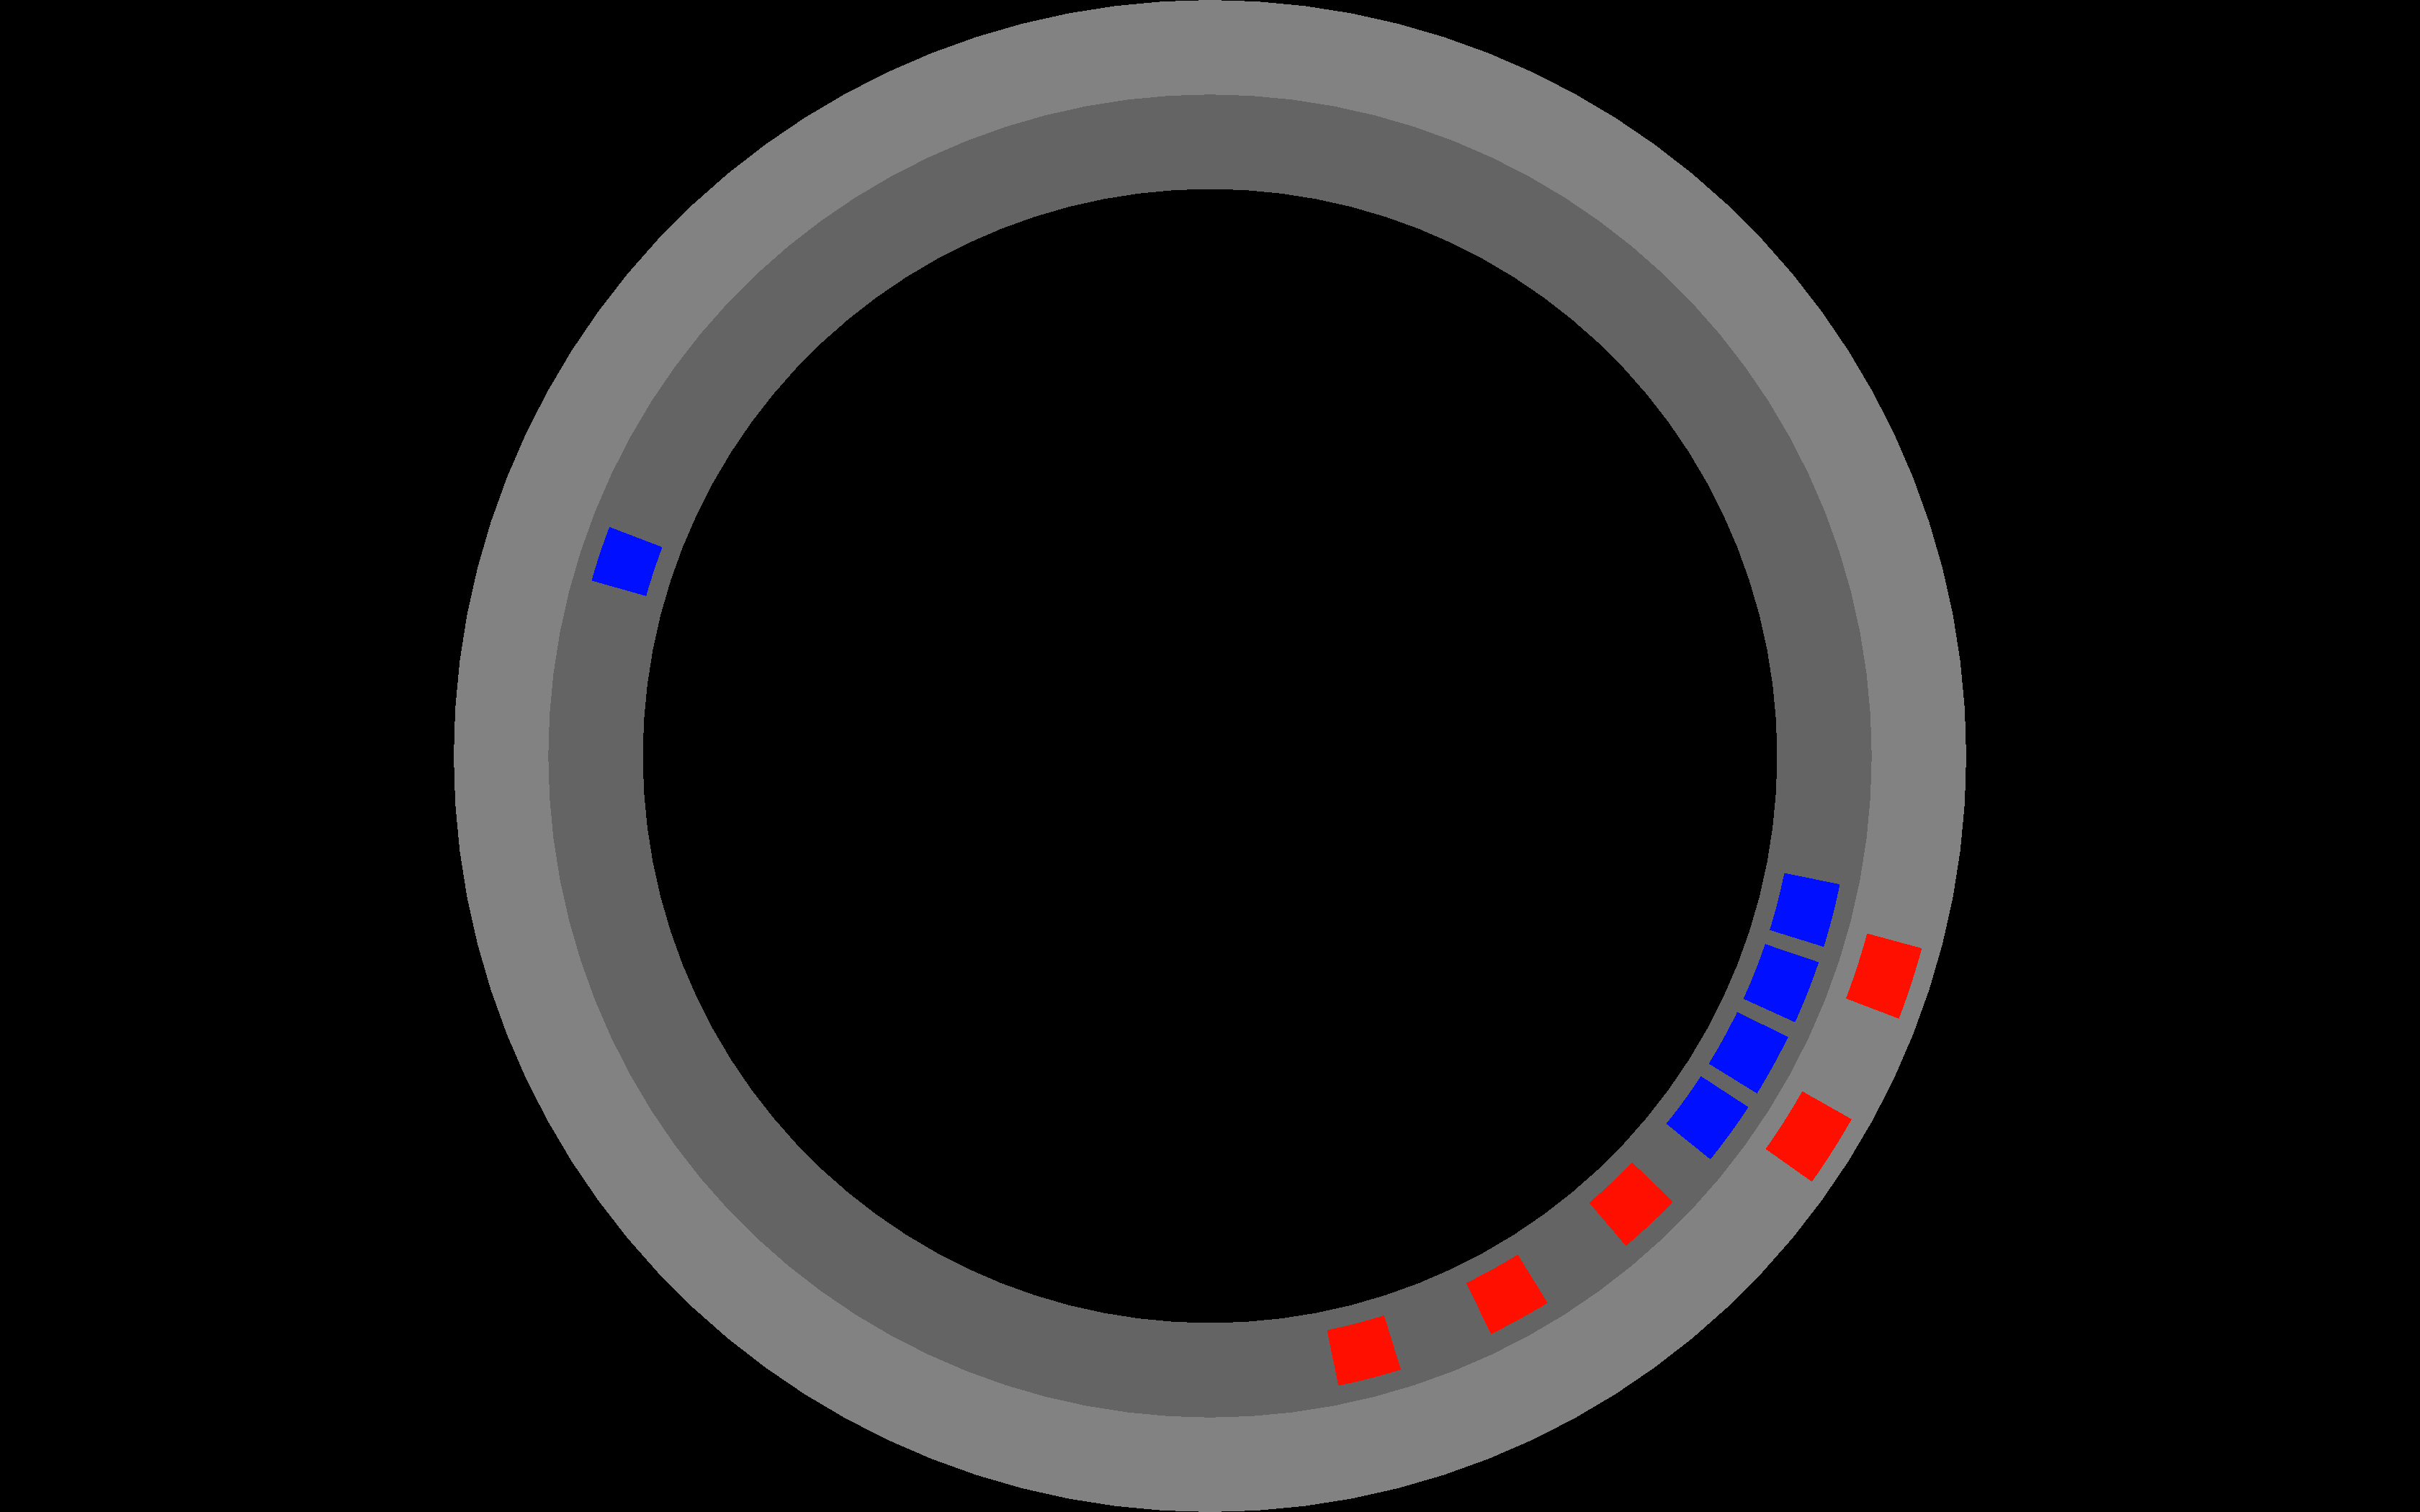
\includegraphics[scale=0.2]{11.png}
	\end{figure}
\end{frame}

\begin{frame}
	\frametitle{Entrada}
	\begin{center}
		\texttt{\$ ./ep2 d n [v|u] [-v]}
	\end{center}	
	\begin{itemize}
		\item \texttt{d}: número inteiro que representa o comprimento em metros da pista.
		\item \texttt{n}: número de ciclistas em cada equipe. 
		\item \texttt{v}: usado para definir simulações com velocidades aleatórias a cada volta. 
		\item \texttt{u}: define simulações com velocidades uniformes de 60 km/h.  
		\item \texttt{-v}: opção para mostrar tudo (debug), utilizado para produzir saída para o terminal. 
	\end{itemize} 
\end{frame}

\begin{frame}
	\frametitle{Saída}
	\begin{itemize}
		\item A saída tem a seguinte forma:
		\begin{figure}[!h]
			\centering
			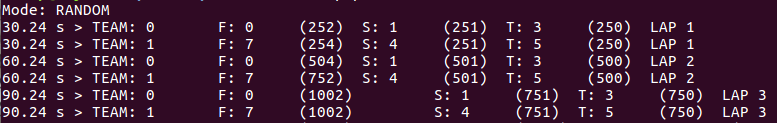
\includegraphics[scale=0.4]{5-a.png}
		\end{figure}
		\item Mostrando o modo das velocidades, e a cada volta (tempo), o primeiro, o segundo e o terceiro colocado de cada time, com a sua metragem percorrida (por 16 voltas).
		\begin{figure}[!h]
			\centering
			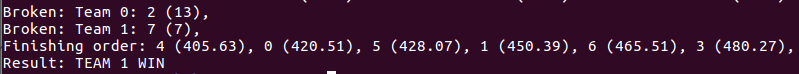
\includegraphics[scale=0.4]{5-b.png}
		\end{figure}
		\item No final, mostra os ciclistas quebrados (número do ciclista e volta que quebrou), a ordem de chegada (número do ciclista e tempo) e quem venceu ou se houve empate.
	\end{itemize}
\end{frame}
	
\begin{frame}
	\begin{itemize}
		\item Se o resultado impresso na imagem fosse \texttt{TEAM 1 WIN*}, isso significa que o terceiro dessa equipe passou o terceiro da outra equipe durante a corrida.
		\item No modo debug, temos as seguintes informações (respectivamente): o número do ciclista, seu time, a distância percorrida na volta, o status, qual pista ele está (interna ou externa), a distância total percorrida e a volta.
		\begin{figure}[!h]
			\centering
			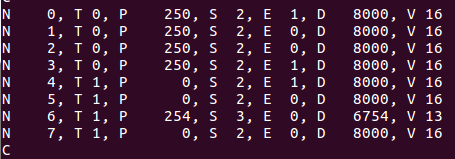
\includegraphics[scale=0.5]{6.png}
		\end{figure}
	\end{itemize}
\end{frame}

\begin{frame}
	\frametitle{Testes}
	\begin{itemize}
		\item Para os testes, utilizamos as seguintes máquinas:
		\begin{figure}[!h]
			\centering
			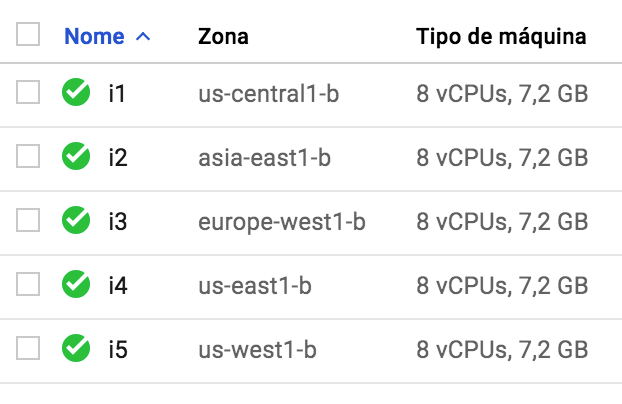
\includegraphics[scale=0.37]{13.png}
		\end{figure}
		\item O uso de CPU ficou assim:
		\begin{figure}[!h]
			\centering
			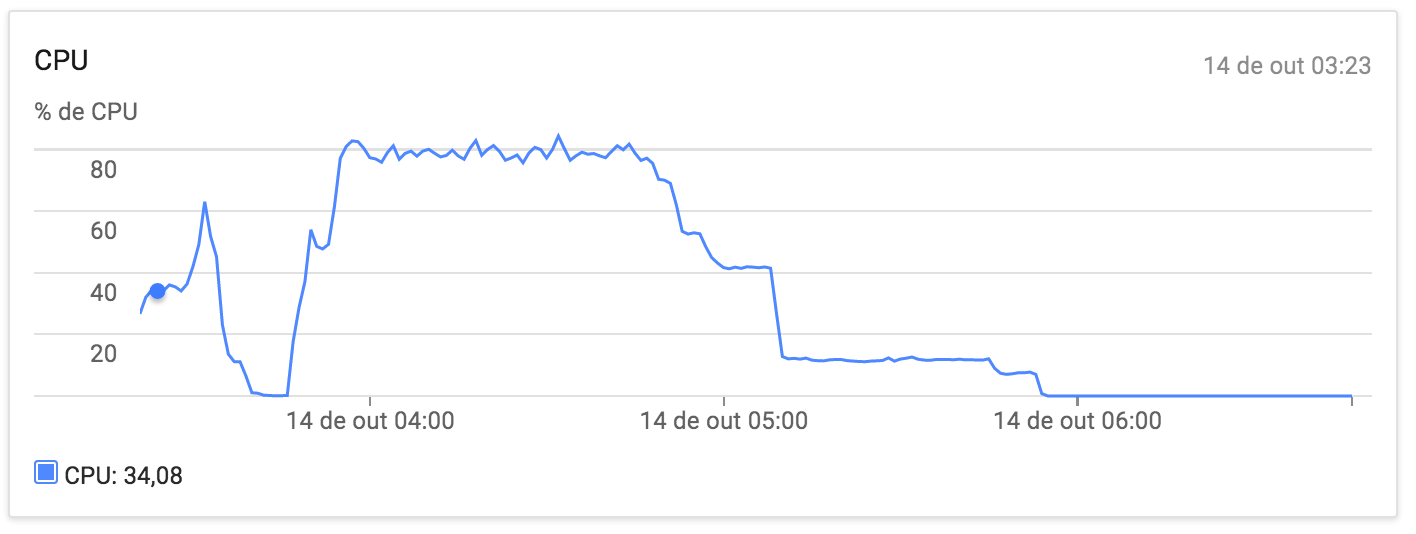
\includegraphics[scale=0.37]{12.png}
		\end{figure}
	\end{itemize}
\end{frame}

\begin{frame}
	\begin{itemize}
		\item Executamos o programa da seguinte maneira:
		\item \quad \texttt{\$ /usr/bin/time -v ./ep2 d n v}
		\item Com isso, temos uma saída desse tipo, além da saída do programa:
		\begin{figure}[!h]
			\centering
			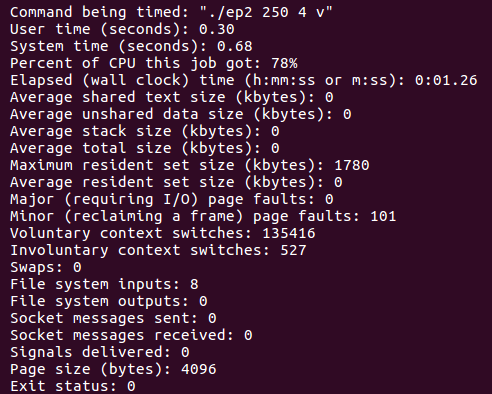
\includegraphics[scale=0.4]{4.png}
		\end{figure}
	\end{itemize}
\end{frame}

\begin{frame}
	\begin{itemize}
		\item De todos esses dados, utilizamos o Maximum resident set size para fazer as medições de uso de memória.
		\item Esse item representa o máximo de memória que pertenceu ao processo e ficou na RAM durante a execução, em kbytes.
		\item Para o tempo de execução do processo, utilizamos o User time, que é o tempo que o processo dura na visão do usuário, em segundos.
		\item Com isso, temos os seguintes gráficos, com poucos (5), muitos (80) e um valor intermediário de ciclistas (20) para uma pista pequena (250 m), média (1000 m) e grande (4000 m).
	\end{itemize}
\end{frame}

\begin{frame}
	\begin{figure}[!h]
		\centering
		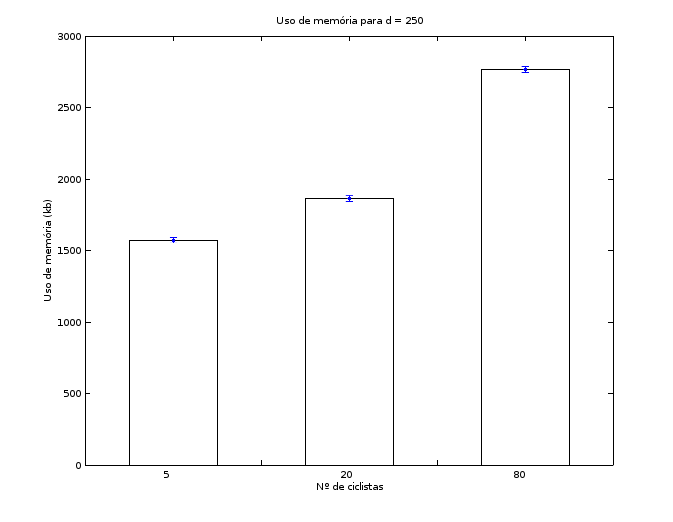
\includegraphics[scale=0.4]{1.png}
	\end{figure}
\end{frame}

\begin{frame}
	\begin{figure}[!h]
		\centering
		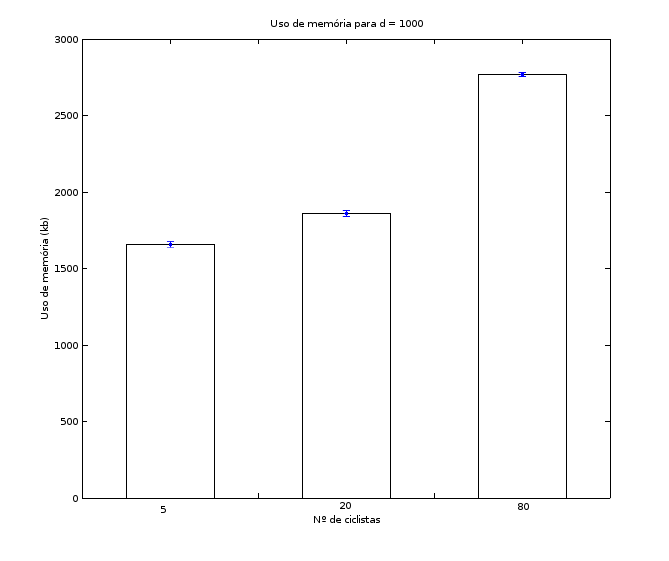
\includegraphics[scale=0.4]{2.png}
	\end{figure}
\end{frame}

\begin{frame}
	\begin{figure}[!h]
		\centering
		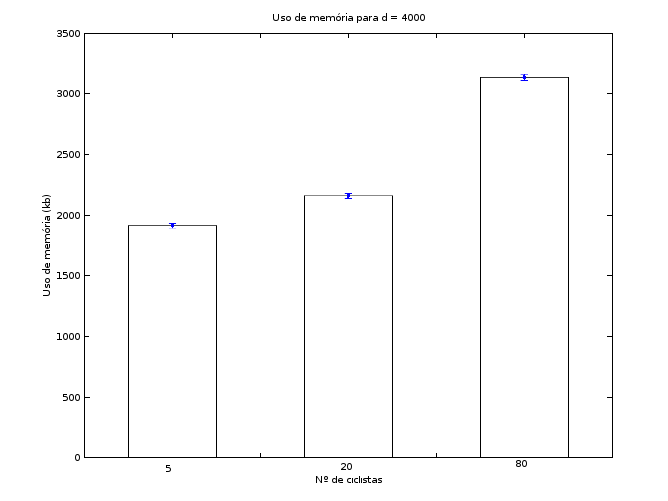
\includegraphics[scale=0.4]{3.png}
	\end{figure}
\end{frame}

\begin{frame}
	\begin{figure}[!h]
		\centering
		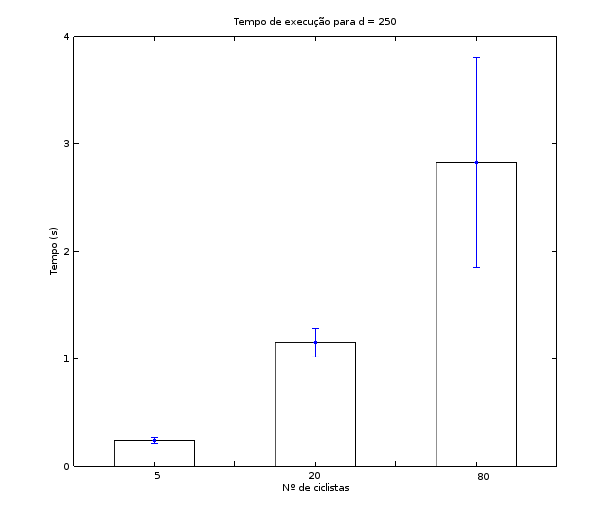
\includegraphics[scale=0.4]{7.png}
	\end{figure}
\end{frame}

\begin{frame}
	\begin{figure}[!h]
		\centering
		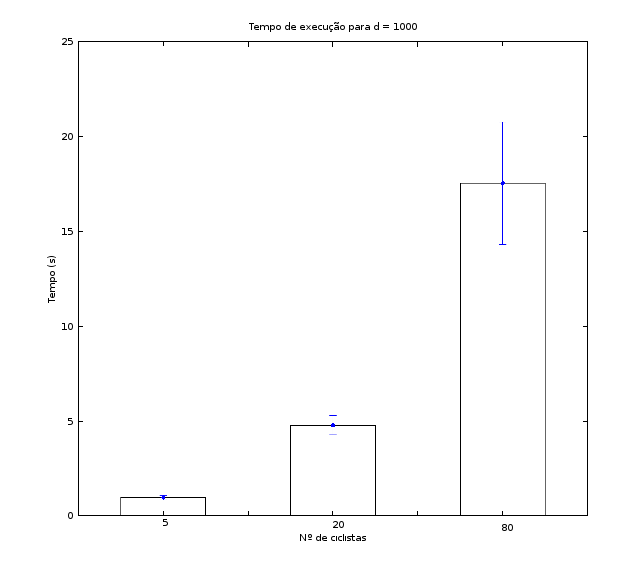
\includegraphics[scale=0.4]{8.png}
	\end{figure}
\end{frame}

\begin{frame}
	\begin{figure}[!h]
		\centering
		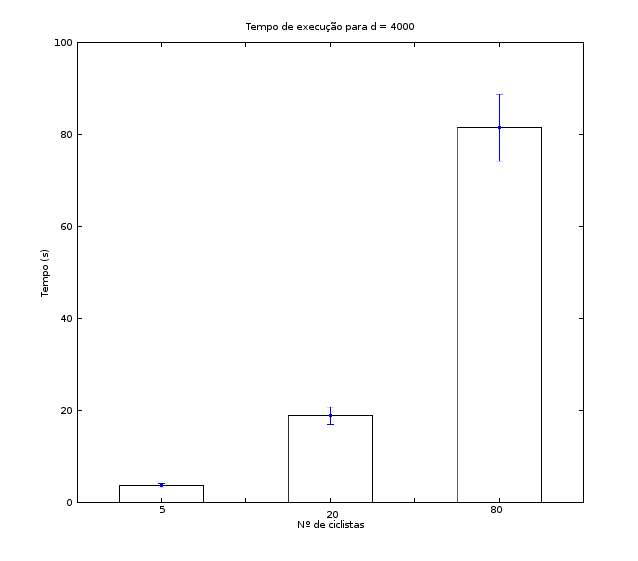
\includegraphics[scale=0.4]{9.png}
	\end{figure}
\end{frame}

\begin{frame}
	Feito por:
	\begin{itemize}
		\item Gabriel Capella, 8962078.
		\item Luís Felipe de Melo, 9297961.
	\end{itemize}
	
\end{frame}

\end{document} 